\cleartooddpage[\thispagestyle{empty}]

\newcommand{\Lim}[1]{\raisebox{0.5ex}{\scalebox{0.8}{$\displaystyle \lim_{#1}\;$}}}
\renewcommand{\labelitemi}{\textbullet}
\newcommand{\pip}[1]{$\pi^{+}$}
\newcommand{\pim}[1]{$\pi^{-}$}
\newcommand{\pio}[1]{$\pi^{0}$}
\newcommand{\sv}{\left < \sigma v \right >}

\chapter{Gamma Rays and Dark Matter}\label{ch_gamma}


This analysis searches for dark matter using gamma rays, thus a discussion of gamma rays and their properties is necessary.
In this chapter, three different topics are discussed.
The first is the astrophysical mechanisms that produce gamma rays.
The second is how dark matter around the Galactic Center can produce gamma rays.
The third topic is how gamma rays induce air showers in the Earth's atmosphere.

\section{Production of TeV Gamma Rays}

  There are several mechanisms that can produce photons with TeV energies.
  A gamma ray can start as a low-energy photon, then gain significant energy from electroweak interactions with electrons, referred to as a leptonic production.
  Alternately, a gamma ray can be created from a high-energy proton colliding with another proton, referred to as hadronic production.
  The primary mechanism this analysis searches for is the annihilation of two WIMP dark matter particles that either directly or indirectly produce gamma rays, and is discussed in Section~\ref{dm_spectral}.

  In leptonic production, electrons and low-energy photons collide, transferring energy to the photon.
  This interaction is called upscattering or inverse Compton scattering~\cite{compton_effect}.
  In inverse Compton scattering, a charged particle interacts with a photon, and some the electron's kinetic energy is transferred to the photon, shifting it to a higher frequency.
  The feynman diagram for this interaction can be seen in Figure~\ref{fig:inv_compt_feyn}.
  
  \begin{figure}[ht]
    \centering
    \includegraphics[width=0.45\textwidth]{images/feynman_particles/inversecompton.pdf}
    \caption[Inverse Compton Scattering Feynman Diagram]{
      Feynman diagram of inverse Compton scattering, where an electron upscatters a low-energy photon (red) to produce a higher-energy (blue) photon.
    }
    \label{fig:inv_compt_feyn}
  \end{figure}
  \FloatBarrier
  
  In inverse Compton scattering, a field of photons with an electron present will gain energy according to Equation~\ref{eqn:inv_compt_en_gain_rate}~\cite{inv_compt1,inv_compt2},
  
  % https://eud.gsfc.nasa.gov/Volker.Beckmann/school/download/Longair_Radiation3.pdf equation 11
  \begin{equation}\label{eqn:inv_compt_en_gain_rate}
    \frac{dE}{dt} = \frac{4}{3} \: \sigma_{\perp} \: U \: c \: \gamma^2 \: \frac{ v^2 }{ c^2 } \;\; .
  \end{equation}

  In Equation~\ref{eqn:inv_compt_en_gain_rate}, 
  \begin{itemize}
    \item $\sigma_{\perp}$ is the perpendicular cross section between the photon and the charged particle, 
    \item $c$ is the speed of light in vaccum,
    \item $\gamma$ is the Lorentz factor,
    \item $U$ is the energy density of the photon field in the rest frame of the electron (e.g. $Uc=N\hbar \omega c$), and 
    \item $v$ is the velocity of the electron in the laboratory frame.
  \end{itemize}

  The average energy $E_{up}$ of photons upscattered this way can be calculated with Equation~\ref{eqn:inv_compt_avg_up_en},
  
  % https://eud.gsfc.nasa.gov/Volker.Beckmann/school/download/Longair_Radiation3.pdf equation 15
  \begin{equation}\label{eqn:inv_compt_avg_up_en}
    E_{up} = \frac{4}{3} \: \gamma^2 \: E_{0} \;\;.
  \end{equation}
  
  % me = 5e5 eV (mass of electron)
  
  % formula for calculating gamma (lorentz factor) from relativistic kinetic energy
  % Ek = mc^2 / sqrt(1-v^2/c^2) - mc^2
  % Ek + mc^2 = mc^2 / sqrt(1-v^2/c^2)
  % ( Ek + mc^2 ) / mc^2 = 1 / sqrt(1-(v^2/c^2)) = g
  
  % lorentz factor for various kinetic energy electrons
  % Ek = 5e5  eV, 500 KeV, g =   2
  % Ek = 1e6  eV,   1 MeV, g =   3
  % Ek = 1e7  eV,  10 MeV, g =  21
  % Ek = 1e8  eV, 100 MeV, g = 201
  % Ek = 1e9  eV,   1 GeV, g = 2e3
  % Ek = 1e10 eV,  10 GeV, g = 2e4
  % Ek = 5e11 eV, 500 GeV, g = 1e6
  
  % calculating the energy in eV of a green photon
  % lg = 550e-9 m  = 5.5e-7 m
  % c = l*w
  % wg = c / lg
  % wg = 2.99e8 m/s / 5.5e-7 m = 5.4e14 1/s
  % E  = hbar w
  % hbar = 1.05e-34 m^2 kg / s (reduced planck constant)
  % 1 J = 6.24e18 eV
  % Eg = hbar wg
  % Eg = 1.05e-34 m^2 kg / s    * 5.4e14 1/s * 6.24e18 eV/J
  % Eg = 1.05 * 5.4 * 6.24 e-34 e14 e18 eV
  % Eg = 35.3e-2 eV
  % Eg = 0.35 eV (energy of a green photon)
  
  % 500 GeV electron upscatters a 0.35 eV photon (green) into a ? eV photon?
  % gamma = (Ek + Ee) / Ee
  % gamma = ( 5e11 eV + 5e5 eV ) / 5e5 eV
  % gamma = 1e6
  % Eup = (4/3) * gamma^2 * Eg
  % Eup = (4/3) * 1e12 * 0.35 eV
  % Eup = 4.67e11 eV = 467 GeV
  
  In Equation~\ref{eqn:inv_compt_avg_up_en}, $E_{0}$ is the energy of the original photon.
  At Earth, astrophysical electrons are detected at energies of \SI{500}{GeV}~\cite{500GeVElectrons}.
  At these energies, the Lorentz factor is $\gamma = 10^6$.
  With this Lorentz factor, upscattered photons can increase their energy by up to\footnote{This is the maximum average energy gain when the upscattered photon is emitted back along its original trajectory.} $\gamma^{2} = 10^{12}$.
  For example, a green photon ($\lambda_{\textrm{green}}=550\,\textrm{nm}$, $E_{\textrm{green}}=0.3\,\textrm{eV}$) could be upscattered to as high as \SI{467}{GeV}, becoming a gamma ray detectable by VERITAS.
  
  In order to efficiently produce gamma rays via this method, a population of high-energy electrons is needed.
  One environment for producing these electrons is around pulsar wind nebulae.
  Because pulsars spin rapidly, they produce strong magnetic fields.
  For example, the pulsar at the heart of the Crab nebula has a surface magnetic field strength of \SI{e12}{G}~\cite{pwn_evolution}, much larger than Earth's $\sim$\SI{0.5}{G}~\cite{earth_geomag}.
  These strong magnetic fields provide an environment for producing and accelerating charged particles.
  In these strong magnetic fields, ambient photons can convert into $e^{+}e^{-}$~\cite{pwn_pairprod2,pwn_pairprod3}.
  The probability $\Upsilon$ (0-1) of a photon pair-converting in a magnetic field is calculated by Equation~\ref{eqn:pwn_pairprod},
  
  \begin{equation}\label{eqn:pwn_pairprod}
    \Upsilon = \frac{E}{mc^2} H \frac{e \hbar}{m^2c^3} \;\;,
  \end{equation}
  
  where $E$ is the photon energy, $H$ is the ambient magnetic field strength, $e$ is the electron charge, and $m$ is the mass of the electron~\cite{pwn_pairprod3}.
  The factor $\frac{e \hbar}{m^2c^3}$ acts as a critical magnetic field strength, which for electrons is $\frac{1}{4.4\times10^{13}\,\textrm{Gauss}}$, similar in scale to the pulsar's surface magnetic field strength.
  
  Charged particles can also be accelerated by a pulsar's magnetic fields, in a process called magnetic reconnection, shown in Figure~\ref{fig:magcon}.
  In this mechanism, two oppositely oriented magnetic fields move towards each other at some velocity (Figure~\ref{fig:magcon}.a), due to the field lines being frozen into the local plasma.
  Because the magnetic field lines are forced to merge (Figures \ref{fig:magcon}.b and c), this causes the ambient plasma in the region to move with the magnetic field lines{\color{red}(??)}.
  This moving plasma then creates electric fields (Figure~\ref{fig:magcon}.d) that can accelerate charged particles~\cite{magcon_crab,magcon_schopper,magcon_review,gamma_pwn1,gamma_pwn2}.
  
  \begin{figure}[ht]
    \centering
    \begin{tabular}{m{1cm}m{10cm}}
      (a) & \includegraphics[width=0.6\textwidth]{images/magnetic_reconnection/diagram_1_cr.pdf} \\
      (b) & \includegraphics[width=0.6\textwidth]{images/magnetic_reconnection/diagram_2_cr.pdf} \\
      (c) & \includegraphics[width=0.6\textwidth]{images/magnetic_reconnection/diagram_3_cr.pdf} \\
      (d) & 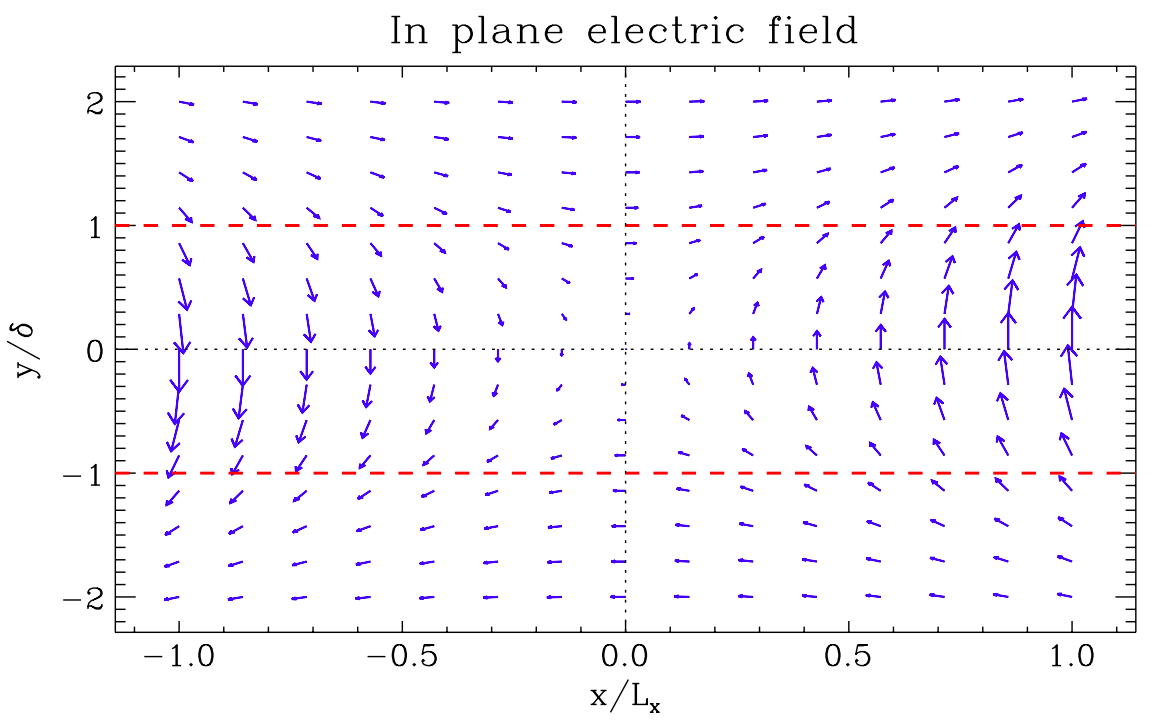
\includegraphics[width=0.6\textwidth]{images/magnetic_reconnection/magcon_efieldlines.pdf}
    \end{tabular}
    \caption[Magnetic Reconnection]{
      Reconnection of two magnetic fields.
      In (a), two oppositely-pointing magnetic fields move into each other.
      In (b), reconnection starts to occur.
      In (c), reconnection occurs, and drags plasma outwards along the $y=0$ axis.
      In (d), the resulting electric fields from the moving plasma are shown in this scenario, from Ref.~\cite{magcon_crab}.
    }
    \label{fig:magcon}
  \end{figure}
  
  
  \FloatBarrier
  % Use figure 2 in http://iopscience.iop.org/article/10.1088/0004-637X/746/2/148/pdf
  
  % Use these sources, to get an idea of the electric field strengths doing the accelerating
  % http://iopscience.iop.org/article/10.1088/0004-637X/746/2/148/pdf
  % https://aip.scitation.org/doi/pdf/10.1063/1.873696
  % https://www.annualreviews.org/doi/pdf/10.1146/annurev-astro-082708-101726
  % something is still missing, can't find complete description of E field
  
  
  
  %The electric field in Figure~\ref{fig:magcon}.d is able to accelerate charged particles, and can be calculated with Equation~\ref{eqn:magcon_efield},
  %\begin{equation}\label{eqn:magcon_efield}
  %  \hat{E} = -\hat{V} \times \frac{B_{z}}{c} \;\; .
  %\end{equation}
  %In Equation~\ref{eqn:magcon_efield}, 
  %\begin{equation}
  %  \hat{V} = \left ( c \frac{x}{L_x} \cosh^{-2} \left ( \frac{y}{\delta} \right ),-c\beta \tanh \left ( \frac{y}{\delta} \right ), 0 \right )
  %\end{equation}
  %From \cite{magcon_crab}, equations (2) and (3).
  % 
  %\begin{equation}
  %  \hat{B} = \left ( B_0 \tanh \left ( \frac{y}{\delta} \right ), \beta B_0 \frac{x}{L_x}, 0 \right )
  %\end{equation}
  %From \cite{magcon_crab}, equations (1) and (4).
  % 
  %But this results in:
  %\begin{equation}
  %  \hat{E} = \left (  0, 0, B_0 \frac{x^2}{L_x} \beta \sech \frac{y}{\delta}^2 - B_0 \beta \tanh \frac{y}{\delta}^2 \right )
  %\end{equation}
  %Which doesn't match the plot in Figure~\ref{fig:magcon}.d .

  Another mechanism that produces high-energy charged particles is fermi acceleration\cite{fermi1949,highenergyelectron_snr}.
  In general, this acceleration imparts energy to charged particles when they are reflected by an oncoming magnetic field.
  
  One environment where this can happen often is in the shockfront of a supernova, where the mechanism is called diffusive shock acceleration~\cite{dsa1,dsa2,dsa3,dsa4,dsa5}.
  During and after a supernova's initial detonation, charged fermions are quickly heated.
  These heated particles then expand outwards, creating a moving shockfront at the boundary between the expanding particles and the surrounding Inter-Stellar Medium (ISM).
  These expanding particles bring their own magnetic fields, which reflect charged particles.
  As the shockfront expands, it also runs into the ambient magnetic fields in the ISM, which can also reflect charged particles.
  This shockfront is shown in Figure~\ref{fig:snr_shockfront}.

  \begin{figure}[ht]
    \centering
    \includegraphics[width=0.75\textwidth]{images/snr_shockfront/shockfront_diagram.pdf}
    \caption[Supernova Shockfront]{
      Diagram of supernova shockfront.
      Relative to some inertial observer, the supernova plasma expands at velocity $v_s$, while the ISM moves at velocity $v_m$.
    }
    \label{fig:snr_shockfront}
  \end{figure}
  
  In this situation, particles that cross the shockfront are reflected off the magnetic fields on the other side, gaining a small amount of energy each time.
  Over many crossings, charged particles can gain high energies, though the higher the energy of the particle, the more likely it can escape the shockfront, since it's gyroradius increases as its energy increases.
  The amount of energy gained is governed by a parameter $\beta$, in Equation~\ref{eqn:snr_beta}, 
  
  \begin{equation}\label{eqn:snr_beta}
    \beta = 1 - \frac{v_s}{c} \;\; .
  \end{equation}
  
  This $\beta$ parameter can be interpreted as the fractional energy gain per crossing, as in Equation~\ref{eqn:snr_beta_en},

  \begin{equation}\label{eqn:snr_beta_en}
    E_{i+1} = \beta E_{i} \;\; .
  \end{equation}
  
  In Equation~\ref{eqn:snr_beta_en}, $E_i$ is the average energy of a charged particle after it's $i^{\textrm{th}}$ crossing.
  The energy gain $\beta$ factor influences the energy spectrum of the escaping charged particles, but so too does the return probability $P$, the probability that the charged particle remains trapped at the shockfront after each crossing.
  This probability $P$ can be calculated with Equation~\ref{eqn:snr_prob}.
  
  \begin{equation}\label{eqn:snr_prob}
    P = 1 - \frac{v_s}{c}
  \end{equation}
  
  With this probability $P$ and the energy gain $\beta$, the energy spectrum of particles that permanently escape the shockfront can be calculated with Equation~\ref{eqn:snr_spec}.
  
  \begin{equation}\label{eqn:snr_spec}
    \frac{dN}{dE} \approx E^{ \frac{\log P}{\log \beta} - 1 }
  \end{equation}
  
  With Equations~\ref{eqn:snr_prob} and \ref{eqn:snr_beta}, the spectrum from Equation~\ref{eqn:snr_spec} can be simplified.

  \begin{equation}\label{eqn:snr_simplify}
    \begin{split}
       \log P     & = \log \left ( 1 - \frac{v_s}{c} \right ) \approx - \frac{v_s}{c} \\
       \log \beta & = \log \left ( 1 + \frac{v_s}{c} \right ) \approx + \frac{v_s}{c} \\
    \end{split}
  \end{equation}
  
  Equation~\ref{eqn:snr_spec} then simplifies to
  
  \begin{equation}\label{eqn:snr_spec_final}
    \begin{split}
      \frac{dN}{dE} & \approx E^{ \frac{\log P}{\log \beta} - 1 } \\
                    & \approx E^{ \frac{ -\frac{v_s}{c} }{ +\frac{v_s}{c} } - 1 } \\
                    & \approx E^{ -1 - 1 } \\
      \frac{dN}{dE} & \approx E^{ -2 } \;\; .
    \end{split}
  \end{equation}

  In Equation~\ref{eqn:snr_spec_final}, the exponent is often referred to as the spectral index $\gamma$.
  From this diffusive shock acceleration, the spectral index of charged particles is approximately -2.
  This is quite close to the observed extragalactic cosmic ray spectrum range of 2-2.2, but additinal effects may soften this index to get to the observed galactic cosmic ray spectrum of $\approx{}3.7$~\cite{cosmicrayspectrumorigin}.
  The spectral index's dependence on $P$ and $\beta$ is shown in two plots in Figure~\ref{fig:snr_spectrum}.
  The top plot in Figure~\ref{fig:snr_spectrum} shows how changing $\beta$, the energy gain per shockfront crossing cycle, and the bottom plot shows the differential spectra with the spectral indicies from the top plot.
  From these two plots, it can be seen that increasing the energy gain per crossing cycle $\beta$ creates a harder spectrum of particles with more higher energy particles, since they can reach escape energies in fewer cycles.
  It can also be seen that trapping more particles at the shockfront (higher $P$) also creates a harder spectrum of escaping particles, as particles can be contained for more cycles, gaining more energy before escaping~\cite{dsa6}.

  \begin{figure}[ht]
    \centering
    \includegraphics[width=0.8\textwidth]{images/snr_shockfront/snr_spectrum.pdf}
    \caption[Supernova Diffuse Acceleration Spectral Indicies]{
      The top plot shows the spectral indicies produced by various combinations of $\beta$, the fractional energy gained by a particle in one crossing cycle (upstream $\rightarrow$ downstream $\rightarrow$ upstream), and $P$, the average chance a particle isunable to escape the shockfront.
      The contours for three spectral indicies $\gamma$ are shown.
      For example, at the orange triangle, each crossing cycle increases a particles energy by a factor of 1.10, while it has a 90\% chance of being permanently trapped, which produces particles with a spectral index of $\gamma=-2.1$.
      The bottom plot shows the differential flux produced by power laws with the three spectral indicies shown in the top plot.
    }\label{fig:snr_spectrum}
  \end{figure}
  
  \FloatBarrier
  
  % slides on supernova shockwaves
  % https://isapp2012paris.sciencesconf.org/conference/isapp2012paris/Stefano_Gabici_three.pdf
  
  % Drury, 2012, "Origin of Cosmic Rays"
  % https://doi.org/10.1016/j.astropartphys.2012.02.006
  % Diffusive shock acceleration, 
  
  % https://www.annualreviews.org/doi/pdf/10.1146/annurev.aa.22.090184.002233 , pg 435:
  %   2 shockfronts, travelling at v1 and v2= v1 * 3/4
  %   v1 = B1 * c # velocity of the collisionless shockfront (just the B fields)
  %   v2 = B2 * c # velocity of the gas particles
  %   1 crossing cycle = reflect off each shock once = E * B2 * 4/3 increase in particle energy
  %   particle tends to escape after (B1-B2)*1/4 crossing cycles


  Protons accelerated in the manner form the majority of the showers detected by the VERITAS telescope, forming an irriducible background in the galactic center observations.
  This background is irriducible due to the fact that proton and gamma-ray air showers are very similar.
  
  After either of these processes produce electrons with high energies, these electrons can then upscatter ambient photons to TeV energies.
  Additionally, electrons spiralling through magnetic fields can produce synchrotron photons at X-ray energies, meaning fewer upscatters are needed to reach TeV energies~\cite{self_compton}.

  In hadronic processes, protons can be accelerated ($p_{accel}$) by Fermi acceleraton, by a supernova remnant~\cite{proton_snr_accel}, or as part of an active galactic nucleus jet~\cite{hadronic1,hadronic2}.
  Then, upon striking an ambient proton ($p_{ambient}$), the interaction will produce $\pi^{+}$, $\pi^{-}$, $\pi^{0}$, and other particles~\cite{pp_pion,pp_pion2,pp_pion3}.
  While other products from the $pp$ interaction may also produce gamma rays, the $pi^0$ decay is the dominant production channel.
  
  \begin{equation}\nonumber
    p_{accel} + p_{ambient} \rightarrow \pi^+ + \pi^+ + \pi^0 + X
  \end{equation}

  The $\pi^{0}$ then quickly (\SI{8.5e-17}{s}~\cite{pdg2016}) decays into two gamma rays.
  Because each pion resulting from the original $pp$ interaction tends to receive $\frac{1}{3}$ of the original proton's kinetic energy, and the $\pi^0$ decays into two gamma rays, each gamma ray ends up with \nicetilde$15\%$ of the original proton's kinetic energy.
  In the rest frame, the $\pi^0$ has a mass of \SI{135}{\MeV}~\cite{pdg2016}, so each photon ends up with \SI{67.5}{\MeV}.
  {\color{red}(what does it say about the photon energy distribution? Can you say something about the photon energy ranges expected, given that the protons are usually of energy this or that?? -orel) (try looking at "Cosmic Gamma Rays" by Stecker, 1971 for an idea of the gamma-ray energy distribution)}
  
  Much of the diffuse gamma-ray component of the galactic disk is due to extra-galactic high-energy protons colliding with the protons of the galactic plane~\cite{GalacticDiffuseGammaRays,extragalactic_agn}.
  Active galactic nuclei posess particle jets, which can accelerate particles when the jet shocks into the extragalactic medium.

  \subsection{Dark Matter Interactions}\label{dmgammaproduction}
    
    The general dark matter particle searched for in this thesis is a WIMP.
    This WIMP may be detectable by three general search schemes, illustrated in Figure~\ref{fig:3_searches}.

    % add popular figure for the three detection type
    \begin{figure}[ht]
      \centering
      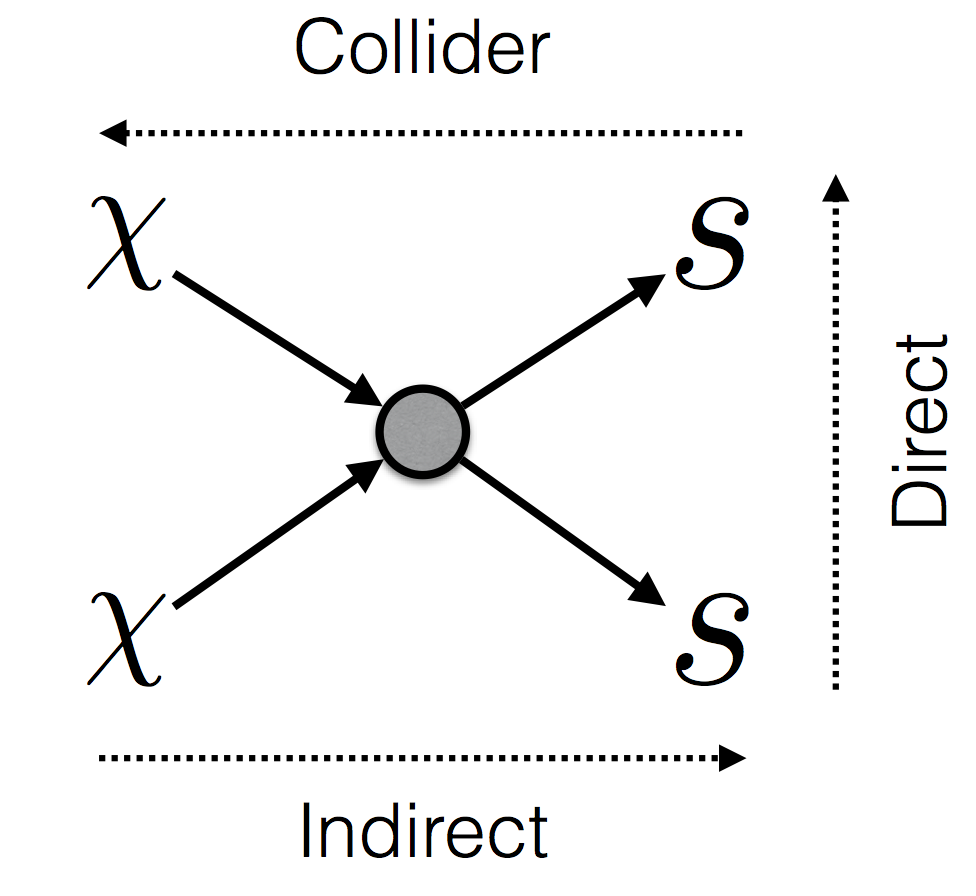
\includegraphics[width=0.65\textwidth]{images/3waystodetect/3waystodetect.pdf}
      \caption[Three Search Techniques]{
        The three general search techniques for dark matter.}
      \label{fig:3_searches}
    \end{figure}
    
    In collider searches, $ss \rightarrow \chi\chi$, standard model particles ($ss$) are accelerated into each other within a detector, and the resulting particle fragments are measured by a slew of detectors~\cite{atlas,cms}.
    These detectors include scintillation crystals with avalanche photodiodes and silicon strip detectors.
    Some of these detectors are within magnetic fields that curve charged particles, aiding in their measurement.
    Since the initial particles are accelerated to known energies, and the output fragment particles are well measured, searching for any break from conservation laws may hint at dark matter particles. 
    
    For direct searches, $\chi s \rightarrow \chi s$, sensitive particle detectors are built deep underground.
    When a WIMP scatters off of a nucleus within the detector, the nuclear recoil can be observed, through signals such as crystal phonons, excitation and release of photons, or ionization.
    Being underground shields the detectors from cosmic rays, which create background collisions that can mimic WIMP signals.
    In liquid Xenon detectors, particle collisions in the liquid produce UV photons and electrons, which are used to infer the presence of WIMPS~\cite{direct_lux,direct_xenon}.
    Cryogenic detectors use pucks of germanium and silicon to measure particle collisions.
    These collisions produce detectable ionization and phonon signals, which are used to classify the incident particle~\cite{direct_cdms}.
    Scintillation detectors are built with crystals like titanium-doped sodium iodine.
    When an external particle collides with one of the nuclei within the crystal, that nucleus becomes excited, and then relaxes by releasing a photon~\cite{direct_dama}.
    However, to date no substantial dark matter signal has been detected with these methods~\cite{direct_dm_detection}.
    
    For indirect searches, $\chi\chi \rightarrow ss$, dark matter particles may annihilate or decay into standard model particles.
    Observatories then search for excesses of these particles, excesses that cannot be explained by known astrophysics.
    This analysis searches for an excess of gamma rays, as the center of our galaxy is believed to host a dark matter halo.
    This spherical halo would allow for many $\chi\chi$ annihilations, producing gamma rays via: 
    
    $$\chi\bar{\chi} \rightarrow S\bar{S} \rightarrow \gamma\gamma$$

    where $S\bar{S}$ can be any quark or lepton particle-antiparticle pair ($t\bar{t}$, $s\bar{s}$, $e^{-}e^{+}$, etc).
    These different annhilation channels can produce different spectra of gamma rays, which will also vary based on the WIMP mass and cross section chosen.
    This is described further in Section \ref{dm_spectral}.

\FloatBarrier

\section{Galactic Center}
  
  The Galactic Center is a complex region of space, with many astrophysical sources of gamma rays.
  At its heart is a supermassive black hole around which is gamma-ray emission, though the production mechanism is not well understood.
  There are other gamma-ray sources as well, including dust along the galactic plane, supernova remnants, and inverse compton emission.
  
  The central black hole has a mass of \SI{4e6}{ \Msol{} }~\ref{sgra_massdist}.
  When observed by TeV-gamma-ray observatories like VERITAS, H.E.S.S., and MAGIC, gamma-ray emission is observed~\ref{gc_pointsrc_hess,gc_veritas_pointsource,VeritasGCRidge2015,hesspsf,gc_hess_2015,gc_magic_2017}
  The VERITAS observations are shown in Figure~\ref{fig:veritas_gc_ridge}.
  
  \begin{figure}[ht]
    \includegraphics[width=0.85\textwidth]{images/veritas_gc_ridge/ridge.pdf}
    \caption[VERITAS View of the Galactic Center Ridge]{
      Galactic Center Ridge
      \CaptionBlankLine
    }
    \label{fig:veritas_gc_ridge}
  \end{figure}
  
  
  * 4e6 \Msol black hole
  * central gamma-ray point source
    * proton pevatron -> pions, or
    * millisecond pulars
    * summary of pevatron or pwn debate \ref{gc_pev_or_pwn}
  * protons collide with dust in galactic plane
  * supernova remnants
  * inverse compton: electrons upscatter photons
  * fermi may see dm halo \ref{gc_fermi_dm}



  {\color{red}(The structure of this section is strange. You start by giving 3 examples of the gamma-ray sources there. Then you describe only two of them in more detail, with some repetitions of the intro. I suggest you re-write. Maybe move the black hole to the intro and then give a short description of all three gamma-ray sources in their own sub-sub-sections. -orel ??)}

  %The Galactic Center is a complex region of space, with many astrophysical sources of gamma rays.
  {\color{red}(Maybe help the reader understand you are listing a few sources of gamma rays from the GC? It reads a little clunky as it is, took me until I reached the end to understand you are giving examples. ?? -orel)}
  A disk of dust lies along the galactic plane, acting as an interaction medium for diffuse proton cosmic rays.
  Nearby supernova remnants also produce gamma rays as their expanding shells interact with ambient dust.
  The immediate area surrounding the Galactic Center contains a point-source gamma-ray emitter, although its mechanism is poorly understood.

  % black hole
  Through kinematic observations of nearby stars, it has been inferred that the Galactic Center is home to a supermassive black hole, with a mass of \SI{4e6}{ \Msol{} }~\cite{sgra_massdist}.
  The Galactic Center is also a source of TeV gamma rays~\cite{gc_pointsrc_hess,gc_pointsource_hess2,gc_veritas_pointsource,gc_magic_pointsource}, though the mechanism that produces them is still under debate.
  One possibility is that the supermassive black hole accelerates protons to PeV energies, which then collide with local atoms to produce $\pi^0$s, which then decay into TeV gamma rays~\cite{gc_pevatron}.
  The second possibility suggests a nearby population of pulsar wind nebulae may be accelerating electrons, which then upscatter local photons to TeV energies~\cite{gc_pulsars}.
  Due to their limited angular resolution, the current generation of gamma-ray telescopes can only resolve the Galactic Center's gamma ray emission as a point source~\cite{VeritasGCRidge2015,gc_pointsrc_hess}.

  The disk of gas present in the galactic plane acts as an interaction medium for passing protons, both from nearby galactic accelerators and from extragalactic sources.
  The interactions between this disk of gas and protons produce $\pi^0$s, which decay into $\gamma\gamma$ pairs~\cite{hess_gc_diffuse}.
  This emission is not modeled in this analysis, because atmospheric effects overwhelm any diffuse emission in the residual skymaps\footnote{These residual maps are discussed in Section~\ref{subsec:likemax}.}.


\section{Indirect Dark Matter Search}
  For this analysis, it is necessary to understand how a terrestrial telescope can detect the presence of dark matter.
  Imaging atmospheric Cherenkov telescopes like H.E.S.S., MAGIC, and VERITAS can indirectly search for dark matter.
  In these searches, these observatories detect gamma rays that are emitted when two dark matter particles annihilate.
  Because the rate of annihilation depends on the local dark matter density, the radially-dependent structure of dark matter halos also affects the gamma-ray emission rate.

  \subsection{Dark Matter and Gamma Rays}
    Primarily, indirect searches focus on annihilating WIMPs, as the predicted decaying WIMP produces a lower flux of standard model particles than annihilation.
    WIMPs may annihilate into any standard model particle-antiparticle pair, but most studies examine a WIMP annihilating into a quark-antiquark or gamma-ray photon pair.
    For example, two annihilating WIMPs may produce a $t\bar{t}$ pair, which then decays into $W^+bW^-\bar{b}$~\cite{pdg2016}.
    Alternately, other pairs may be produced, like  $b\bar{b}$, $c\bar{c}$, $W^+W^-$, $u^+u^-$, or $\tau^+\tau^-$.
    These different annihilations produce different spectra of final gamma rays.
    The final spectrum of gamma rays used in this analysis is calculated in Section~\ref{dm_spectral}.
  
  \subsection{Dark Matter Halo Structure}\label{dm_spatial}
    
    Observations allow most galactic dark matter halos to be modeled using a class of similar density profiles.
    A currently favored profile is the Einasto profile~\cite{einastoprofile1,einastoprofile2}.
    This profile describes the mass-density of dark matter at a distance $r$ from the halo center, $\rho(r)$.
    The Einasto profile is described by Equation~\ref{eqn:einasto}:

    \begin{equation} \label{eqn:einasto}
      \rho_{\textrm{DM}} \left( r \right) = \rho_{s} Exp \left( - \frac{2}{\alpha} \left( {\left( \frac{r}{r_s} \right)}^{\alpha} - 1 \right) \right) \;\; .
    \end{equation}
    
    
    In Equation~\ref{eqn:einasto}, $r_s$ is the scale radius of the halo, which specifies how wide the dark matter halo is.
    The parameter $\rho_s$ is the scale density, which is the dark matter density at the scale radius.
    The parameter $\alpha$ is the power of the density profile's slope.
    A larger $\alpha$ results in smaller dark matter densities above and below the scale radius $r_s$.
    Both $\alpha$ and $r_s$ are from the best fit values of the Aq-A-1 simulation in Table 2 of Ref.~\cite{mw_halo_params}.
    The $r_s$ parameter is calculated via $r_s=r_{-2}=15.14\:\textrm{kpc}$, where $r_{-2}=\frac{11.05}{h_{73}}\:\textrm{kpc}$ (in Ref.~\cite{mw_halo_params}, Table 2) and $h_{73}=0.73$ from Section 2.1 in Ref.~\cite{mw_halo_params}.
    In the model, the parameter $\alpha$ is fixed to 0.17, and $r_s$ is fixed to \SI{15.14}{kpc}.
    The distance to the galactic center is known to be $r_\odot=8\:\textrm{kpc}$~\cite{gc_distance_1,gc_distance_2,gc_distance_3}.
    The assumed Milky Way mass profile has a mass density of $\rho_\odot = 0.4\:\frac{\textrm{GeV}}{\textrm{cm}^3}$~\cite{local_dm_density,direct_dm_astrophysical_uncertainties}.
    Since $r_\odot$ and $\rho_\odot$ are known, then in Equation~\ref{eqn:einasto} the dark matter density at the scale radius $\rho_s$ is derived to be \SI{0.12}{\GeV\per\cm^3}.
    With these values, the Einasto profile in Equation~\ref{eqn:einasto} is shown in Figure~\ref{fig:gchalo_density}.
  
    \begin{figure}[ht]
      \centering
      \includegraphics[width=0.95\textwidth]{images/halo/gc_einasto_profile.pdf}
      \caption[Galactic Center Einasto Halo Density]{
        Mass density of the Einasto dark matter halo (Equation~\ref{eqn:einasto}) used in this analysis.
        The bottom x axis shows the angle from the Galactic Center, while the top x axis shows the distance in kiloparsecs.
        \CaptionBlankLine
        }
      \label{fig:gchalo_density}
    \end{figure}

    Other density profiles exist, but in this analysis only the Einasto profile is considered.
    Most simulations show that density profiles should terminate in a sharp peak at $r=0$, but observations of dwarf galaxies instead favor a flat core within a given radius~\cite{flores1994observational,CoreVsCusp}.
    This may be due to the presence of baryons in this core region, which can diffuse the central cusp of WIMPs into a core-like shape~\cite{corecusp_baryondiffuse1,corecusp_baryondiffuse2}.
    As this flat core occurs in the innermost region covered by the gamma-ray observations n this analysis, the choice of a cuspy or cored dark matter halo can have a significant impact on this analysis.
    Specifically, if the dark matter halo follows a cored profile when using a cuspy halo model, then any derived upper limits on the dark matter cross section would be different.
    For simplicity, only a cuspy halo is used in this thesis.
    
    When choosing which dark matter target to observe with a gamma-ray observatory, knowing the gamma-ray brightness of different sources can be useful.
    This Einasto density profile can be integrated to calculate this gamma-ray brightness, independent of the WIMP model being searched for.
    For annihilating dark matter, $\rho_{\textrm{DM}}\left(r\right)^2$ must be integrated along the line of sight.
    Equation~\ref{eqn:dmflux} can be used to calculate the amount of gamma rays produced by these annihilations.
    
    \begin{equation}\label{eqn:dmflux}
      \frac{ d\Phi }{ dE d \Omega } = \frac{ \left \langle \sigma v \right \rangle }{8 \pi m_\chi^2} \frac{dN_{\gamma}}{dE} \int \rho^2 dl
    \end{equation}
    
    In this equation, the photon flux $\Phi$ is the number of gamma rays detected per $\textrm{area}\times\textrm{time}$.
    The velocity-averaged cross section of the dark matter candidate is $\left \langle \sigma v \right \rangle$.
    Velocity-averaging is used because the cross section is velocity dependent, and the WIMPs that pass through a volume of space will have a distribution of velocities~\cite{wimp_veldist}.
    The spectrum of photons produced by a single $\chi\chi$ annihilation is $\frac{dN_{\gamma}}{dE}$.
    The density integral in Equation~\ref{eqn:dmflux} is often calculated separately, as in Equation~\ref{eqn:jfactor}, and is referred to as the $J$ factor,

    \begin{equation}\label{eqn:jfactor}
      J = \int \rho^2 dl \;\; .
    \end{equation}

    The $J$ factor is used to compare the relative gamma-ray brightness of different dark matter halos, which is a function of both dark matter density and observing distance.
    The Einasto density in Equation~\ref{eqn:einasto} can be integrated to calculate the $J$ factor at various radii, which is shown in Figure~\ref{fig:gchalo_jfactor}.
    In Figure~\ref{fig:gchalo_jfactor}, the profile shown is calculated with Equation~\ref{eqn:dmflux}, where the $d\Omega$ is integrated in bins of \ang{0.01}.
    This J-factor profile then forms the spatial component of the dark matter halo, $M_{s,\textrm{halo}}$, used in Chapter~\ref{chapter:analysis}.
    The J-factor is shown in a two-dimensional plot in Figure~\ref{fig:halojfactor}.
    
    \begin{figure}[ht]
    \centering
      \includegraphics[width=0.95\textwidth]{images/halo/gc_einasto_jfactor.pdf}
      \caption[Galactic Center Einasto Halo Jfactor]{
        J-factor profile as a function of angle from the Galactic Center, calculated via Equation~\ref{eqn:jfactor} with the Einasto density profile in Equation~\ref{eqn:einasto}.
        The J-factor values are calculated by integrating \ang{0.01} around each angle from the Galactic Center.
      }
      \label{fig:gchalo_jfactor}
    \end{figure}
  
  \begin{figure}[ht]
    \centering
    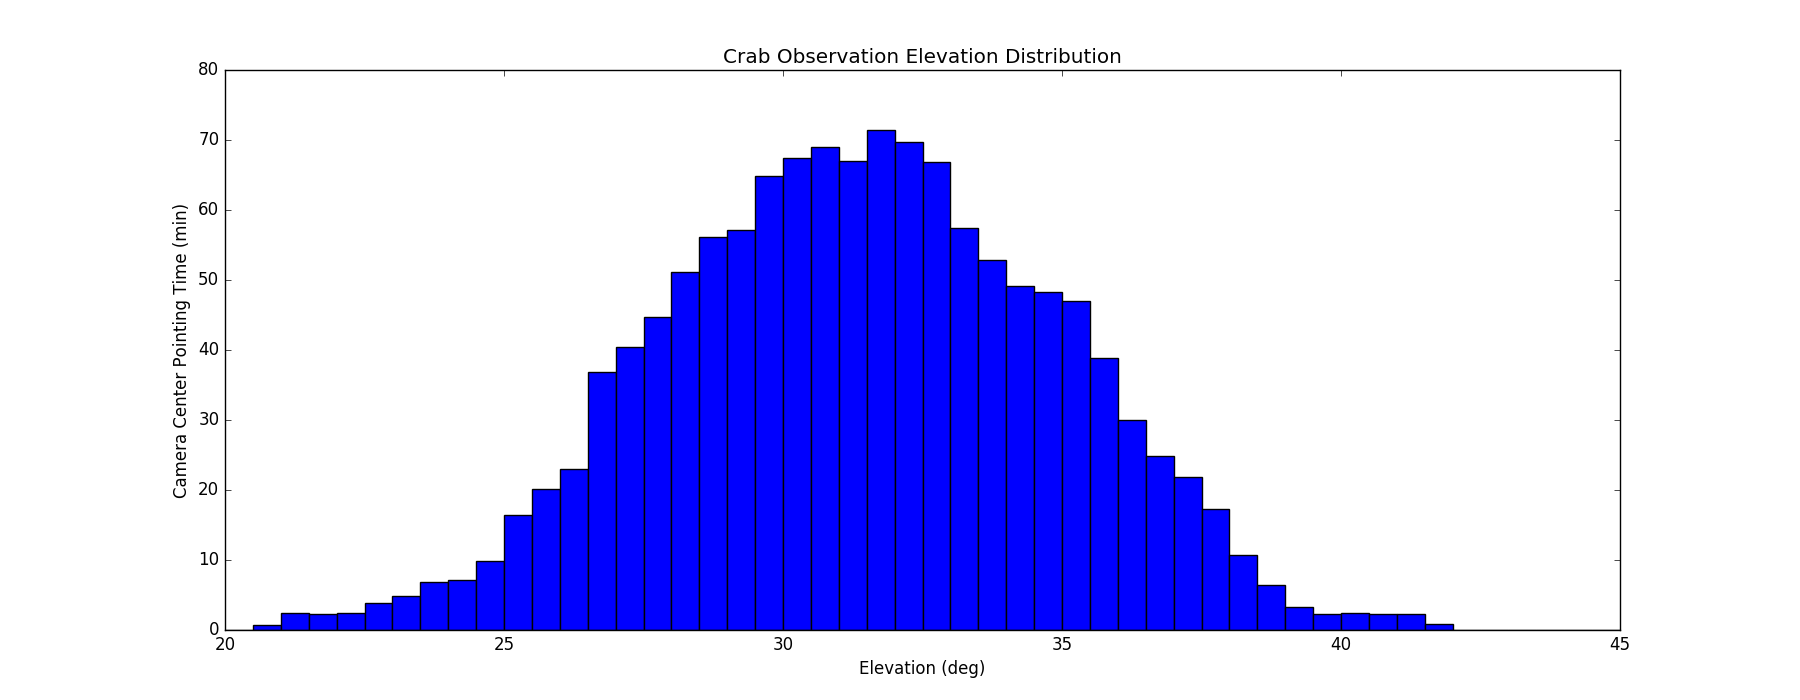
\includegraphics[width=0.95\textwidth]{images/halo_flux/plot.pdf}
    \caption[Galactic Center Halo J-factor Skymap]{
      J-factor of the dark matter halo model used in this analysis.
      The green circles indicate the different observation regions.
      Note this is showing the same model as Figure~\ref{fig:gchalo_jfactor}, except here the J-factor axis is linear instead of logarithmic.
      The black corners result from the halo model only being calculated out to a radius of \ang{3}, since there are no observations that extend past that.
    }
    \label{fig:halojfactor}
  \end{figure}

  The halo structure outlined above is a simple first step halo, one that does not account for more complex dark matter models.
  For example, a search for decaying dark matter would instead change the J-factor calculation to $\int \rho \, dl$, spreading out the gamma-ray emission.
  More exotic WIMP models may slightly alter the gamma-ray brightness of the dark matter halo, compared to the previously mentioned WIMP model.
  For example, if dark matter WIMPs have an attractive force between them, their effective annihilation cross section is enhanced, increasing the gamma-ray emission from the halo.
  This effect is called Sommerfeld enhancement~\cite{sommerfeld}.
  The dark matter search in this thesis does not include this effect.
  % originally from http://inspirehep.net/record/1286230/files/Thesis-2009-Nierop.pdf
  % from http://www.pnas.org/content/112/40/12264.full.pdf
    
  
  \FloatBarrier
  
    
  \subsection{Spectrum of Gamma Rays from Dark Matter}\label{dm_spectral}
    In order to calculate the gamma-ray brightness of the dark matter halo, the produced spectrum from each WIMP annihilation must be known.
    Each WIMP annihilation can have distinct outcomes (each producing different pairs of particles), referred to as annihilation channels.
    WIMPs may annihilate directly into two gamma rays (the $\gamma\gamma$ channel), or may instead produce a quark-antiquark pair ($b\bar{b}$, $t\bar{t}$, ...), a lepton-antilepton pair, or almost any other standard model particle-antiparticle pair.

    Non-gamma-ray annihilation channels may still indirectly produce gamma rays as the original particle pair decays.
    Many standard model interactions also result in a mix of channels, where the same interaction may produce different sets of particles with different probabilities, so WIMP annihilations may also have this feature.
    For an example set of 100 WIMP annihilation pairs, 80 pairs may annihilate into a $t\hat{t}$ pair, but then another 10 pairs may annihilate into a $b\hat{b}$ pair, and the remaining 10 pairs annihilate into other standard model particles.
    However, these mixed-channel searches are beyond the scope of this analysis.
    The software package CLUMPY~\cite{CLUMPYcode} is used to calculate the gamma-ray spectra for each annihilation channel.
    The spectral models that CLUMPY uses are based on the annihilation spectra in the PPPC 4 DM ID~\cite{pppc4_dm_spectra,pppc4_ewcorrections}.
    These spectra are calculated using monte carlo simulations of with PYTHIA~\cite{pythia} and HERWIG~\cite{herwig}.
    For this analysis, only the $b\bar{b}$ annihilation channel is considered.
    Figure~\ref{fig:chichi_spectrum} shows the resultant spectra from the single annihilation of two WIMPs.
    Each line shows the spectrum from a different initial WIMP mass.

    \begin{figure}[ht]
      \centering
      \includegraphics[width=0.95\textwidth]{images/spectra/chichi_spectrum.pdf}
      \caption[Single Annihilation Spectra]{
        Resultant photon spectra from a single annihilation of WIMP particles.
        Each colored line represents a different WIMP mass.
      }
      \label{fig:chichi_spectrum}
    \end{figure}

    These spectra can be combined with the J factor Equation~\ref{eqn:jfactor} to calculate Equation~\ref{eqn:dmflux}: how many gamma rays are produced by the halo\footnote{
      These spectra are then used as the spectral component $M_{\textrm{e,halo}}$ for the dark matter halo model in the likelihood analysis in Equation~\ref{eqn:dmmodel}, detailed further in Section~\ref{subsec:dmhalomodel}.
    }.
    
    Using some estimated parameters with Equation~\ref{eqn:dmflux}, the flux of gamma rays from a dark matter halo can be estimated to understand how few events a dark matter halo produces.
    For this estimate, the dark matter mass is chosen to be \SI{10}{TeV}, and the velocity-averaged cross section $\left < \sigma v \right >$ is set at the relic cross section.
    Other chosen parameters are specified in Table~\ref{tab:halo_nphotons}, to align with the VERITAS telescope performance, or the parameters of the dark matter analysis performed in later chapters.
    For the table parameters, the dark matter halo would only produce a VERITAS-detectable gamma ray between \SIrange{4}{70}{TeV} every 39 hours.
    This flux $\Phi$ is proportional to the $\sv$, so a factor of $n$ larger particle would produce a factor of $n$ larger photon flux.
    It is interesting to note that, if the entire VERITAS energy range of \SIrange{1.5}{70} is used, the Integrated Photon Spectrum increases to 0.13 events per annihilation, increasing the observed photon flux by a factor of 26.
    
    \begin{table}[]
      \centering
      \begin{tabular}{r|l}
        \hline
        \textbf{Estimated Parameters}            & \\
        $m_{\chi}$                               & \SI{10}{TeV}         \\
        relic $\left < \sigma v \right >$        & \SI{3e-26}{cm^3/s}   \\
        Field of View                            & \ang{3}              \\
        Detectable Photon Energy Range           & \SIrange{4}{70}{TeV} \\
        Observatory Effective Area               & \SI{287000}{m^2}     \\
        Annihilation Branch                      & $\chi\chi \rightarrow b\bar{b}$ \\
        DM Halo Shape                            & Einasto              \\
        \hline
        \textbf{Derived Values}                  & \\
        Integrated Photon Spectrum : $\int \frac{dN_{\gamma}}{dE} dE$        & 0.00536 photons per $\chi\chi$ annihilation \\
        J factor :$\int \int \rho^2 dl\,d\Omega$ & \SI{3.88e22}{GeV^2/cm^5}      \\
        Halo Flux $\Phi$                         & \SI{2.5e-11}{photons/(s*m^2)} \\
        One halo photon detected every           & \SI{39}{hours} \\
        \hline
      \end{tabular}
      \caption{
        Number of Gamma Rays from a Dark Matter Halo.
        Field of view is the radial field of view of VERITAS.
        Observatory Effecitve area is the VERITAS effective area at \ang{28} telescope elevation, \ang{0.5} offset from GC, at the $\log_{10}$ mean energy (\SI{16.7}{TeV})in the selected energy range.
        The Einasto halo shape parameters are chosen to be the same as in Section~\ref{dm_spatial}.
      }
      \label{tab:halo_nphotons}
      % values derived with $VERIPY/thesis/analysis/example_dm_halo_photons/example.py
    
    \end{table}

    \FloatBarrier
    
\section{Cherenkov Photons}\label{sec:cherenkov}

  Because the detection of gamma rays in Section~\ref{sec:atmoshowers} relies heavily on knowledge of Cherenkov light, Cherenkov light and its production is discussed here.
  Within the Earth's atmosphere (or any dielectric medium), the phase velocity of light $c_{atmosphere}$ is slightly slower than in a vacuum.
  Any charged particles travelling at velocity $v > c_{atmosphere}$ will induce the atmosphere to produce Cherenkov photons~\cite{cherenkov}.
  From a single charged particle of constant velocity, Cherenkov photons form a conical wavefront shown in Figure~\ref{fig:cherenkovangle}.
  This wavefront is similar to a sonic boom shockwave, or the wake produced when a boat travels faster than the speed of the waves.

  \begin{figure}[ht]
    \centering
    \includegraphics[width=0.27\textwidth]{images/cherenkov_angle/cherenkovangle.pdf}
    \caption[Chernekov Emission Angle]{
      Cherenkov light (blue arrows) is emitted at angle $\theta$, relative to the charged particle z's path.
    }
    \label{fig:cherenkovangle}
  \end{figure}

  Cherenkov photons are produced at an angle $\theta$ relative to the charged particle's path, determined by the index of refraction of the medium $n$, the speed of the charged particle $v$, and the speed of light in the medium $c$, as in Equation~\ref{eqn:cherenkovangle}.
  For the air showers used in this analysis, the Cherenkov angle $\theta$ is \nicetilde\ang{1}.
  % showers are 10km up, light pool on ground is 130m diameter, \theta = ArcSin(130/10000) * 180 / pi = 0.73deg ~ 1deg

  \begin{equation}\label{eqn:cherenkovangle}
    \theta = ArcCos \left ( \frac{c}{n \; v} \right )
  \end{equation}
  
  Actual air showers are more complex, however, because the number and distribution of charged particles and their velocities, as well as energy losses, tend to smear the theoretically-clean Cherenkov cones into a diffuse pool of light on the ground, shown in Figure~\ref{fig:lightpool}.

  \begin{figure}[ht]
    \centering
    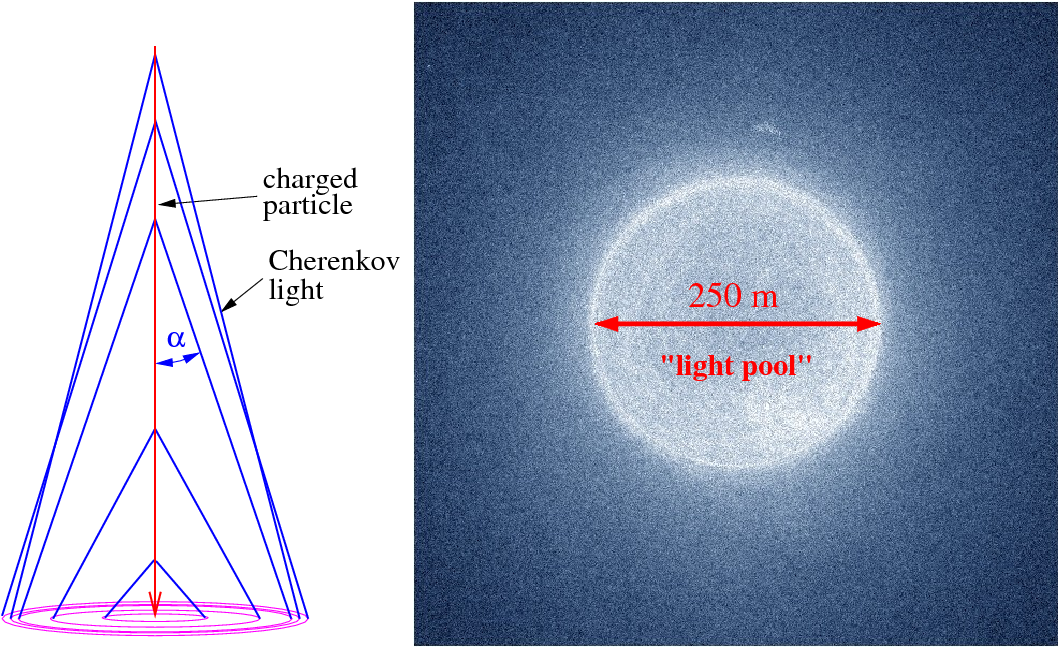
\includegraphics[width=0.85\textwidth]{images/lightpool/lightpool.pdf}
    \caption[Chernekov Light Pool]{
      Cherenkov light from a gamma ray shower illuminating the ground.
      Due to the changing atmospheric density, the Cherenkov angle changes as the electromagnetic shower decends (Left), concentrating the emitted light into a ring-like pool (Right).
      The initial gamma ray had an energy of \SI{1}{\TeV}.
      Figure is from Ref.~\cite{Voelk}.
    }
    \label{fig:lightpool}
  \end{figure}
  
  The spectrum of photons produced by the Cherenkov effect can be calculated with the Frank-Tamm formula~\cite{franktamm1,franktamm2} in Equation~\ref{eqn:franktamm},
  
  \begin{equation}\label{eqn:franktamm}
    \frac{dE}{dx\,d\omega}=\frac{(ze)^2 \, \omega}{c^2} \left ( 1 - \frac{c^2}{v^2 \;\epsilon(\omega)} \right )
  \end{equation}
  
  where $E$ is the energy emitted as Cherenkov radiation, $x$ is the length of the charged particle path, $ze$ is the charge of the particle, $\omega$ is the emitted Cherenkov photon frequency, $c$ is the speed of light (phase velocity) in the medium, $v$ is the speed of the particle, and $\epsilon(\omega)$ is the frequency-dependent permittivity.
  
  \begin{figure}[ht]
    \centering
    \includegraphics[width=0.75\textwidth]{images/CherenkovReactor/cherenkovreactor.eps}
    \caption[Chernekov Light from a Reactor]{
      Blue Cherenkov light in the Advanced Test Reactor core, at the Idaho National Laboratory~\cite{cherenkovreactor,atrlab}.
    }
    \label{fig:cherenkovreactor}
  \end{figure}
  
  In Figure~\ref{fig:cherenkovreactor}, a visible example of Cherenkov photons is shown, produced in the Advanced Test Reactor at the Idaho National Laboratory.
  Neutrons emitted by the reactor collide with atoms in the water, freeing some electrons with enough kinetic energy to travel faster than the speed of light in water.
  These superluminal-in-water electrons then create the blue Cherenkov photons imaged here.
  
  Now that it is understood that Chernekov light is produced by charged particles, the next Section~\ref{sec:atmoshowers} discusses how particles from outer space can produce waves of Cherenkov photons.
  These UV- and visible-spectrum Cherenkov photons are then imaged and recorded by the VERITAS observatory, discussed in Chapter~\ref{chapter:veritas}.
  
    
\section{Atmospheric Showers}\label{sec:atmoshowers}

  When a particle strikes an atom of Earth's atmosphere at GeV or higher energies, it sets off a cascade of energetic particles called an air shower~\cite{Bethe1934,Klein1999}.
  When the primary particle is composed of one or more hadrons, like a proton or iron atom, it creates a hadronic shower.
  When the primary is a gamma ray or a charged lepton, it creates an electromagnetic shower.
  Electromagnetic showers produce a cascade of $e^{\pm}$s and $\gamma$s, where each successive generation of particles tends to have more particles but less energy per particle than the last.
  To start the shower, the primary gamma ray will interact with an atmospheric atom, producing an $e^{-}e^{+}$ pair, each with roughly half the primary gamma ray's energy, as shown in Figure~\ref{fig:emcascade}.
  The $e^{-}$ and $e^{+}$ emit bremsstrahlung photons, and incite the atmosphere to emit Cherenkov photons.
  Cherenkov photon production is discussed further in Section~\ref{sec:cherenkov}.
  The higher-energy bremsstrahlung photons then produce $e^{-}e^{+}$ pairs, which go on to produce more bremsstrahlung and Cherenkov photons.
  As each newly created particle has less energy than its parent particle, eventually the particles in the shower don't have enough energy to produce additional child-particles.
  When electrons have around \SI{80}{MeV} or less of kinetic energy, energy losses due to ionization begin to dominate~\cite{pdg_2014}.

  \begin{figure}[ht]
    \centering
    \includegraphics[width=0.95\textwidth]{images/cascade_diagram/feynman/cascade.pdf}
    \caption[Electromagnetic Cascade]{
      Diagram of the first few generations of an electromagnetic cascade as it decends downwards through the atmosphere, layered by interaction generation~\cite{ellis2017tikz}.
      At the top of the diagram, $\gamma{}_o$ is the initial astrophysical gamma ray.
      \CaptionBlankLine
    }
    \label{fig:emcascade}
  \end{figure}

  Of all detected air showers, \nicetilde{}99\% are due to protons and electrons, rather than gamma rays.
  Protons produce hadronic showers which also produce Cherenkov light, like electromagnetic showers.
  In the initial collision, the astrophysical proton $p_{\textrm{cosmic}}$ interacts with an atmospheric proton $p_{\textrm{atmo}}$.
  The proton-proton collision then produces a set of pions, as in Equation~\ref{eqn:protoncollision}, as well as other particles (`$X$') whose production rates vary with available interaction energy.
  
  \begin{equation}\label{eqn:protoncollision}
    p_{\textrm{cosmic}} + p_{\textrm{atmo}} \rightarrow \pi^+ + \pi^+ + \pi^0 + ...
  \end{equation}
  
  The interaction produces $\pi^+\pi^+\pi^0$, where each particle receives \nicetilde $\frac{1}{3}$ of the initial proton's energy.
  This $\pi^{0}$ decay is shown in Figure~\ref{fig:feynman_pi0}.
  
  \begin{figure}[ht]
    \centering
    \includegraphics[width=0.5\textwidth]{images/feynman_particles/pion_gamma.pdf}
    \caption[Feynman Diagram of $\pi^{0}$ Decay]{
      Feynman diagram of a $\pi^{0}$ decaying into two photons.
      \CaptionBlankLine
    }
    \label{fig:feynman_pi0}
  \end{figure}

  \begin{figure}[ht]
    \centering
    \includegraphics[width=0.5\textwidth]{images/feynman_particles/pionplus.pdf}
    \caption[Feynman Diagram of $\pi^{+}$ Decay]{
      Feynman diagram of $\pi^{+}$ decaying into a lepton pair.
      \CaptionBlankLine
    }
    \label{fig:feynman_piplus}
  \end{figure}
  
  In order to accurately measure the gamma rays from an astrophysical source, the hadronic showers must first be removed.
  Because hadronic showers produce a slightly different image of Cherenkov light, many of them can be excluded from the analysis.
  The process of identifying and excluding these hadronic showers is sometimes known as gamma-hadron separation.

  % see here for neutron: https://en.wikipedia.org/wiki/Cosmic_ray
  In hadronic showers, any produced \pip{}'s and \pim{}'s can travel far in the tranverse direction, away from the main axis of the primary particle.
  The \pip{}'s and \pim{}'s then decay into $\mu^{+}\nu_{\mu}$ and $\mu^{-}\bar{\nu}_{\mu}$ pairs, respectively.
  The \pip{} decay is shown in Figure~\ref{fig:feynman_piplus}.
  The \pio{} quickly decays into pair of gamma rays, each of which then start their own electromagnetic shower.
  The \pip{} and \pim{} have longer decay times ($\pi^{\pm} \rightarrow $\SI{3e-8}{s} vs $\pi^{0} \rightarrow $\SI{9e-17}{s}~\cite{pdg_2014}), allowing them to carry energy farther away from the central shower axis.
  Both of these effects create sub-showers farther away from the primary particle axis, which tends to cause hadronic showers (and their resulting Cherenkov images, discussed in Section \ref{sec:cherenkov}) to be wider than a purely electromagnetic shower of the same length. 
  
  In Figure~\ref{fig:gamma_vs_proton_airshower}, the differences between a gamma-ray shower (left) and a proton shower (right) are shown.
  In the figure, darker areas indicate more Cherenkov photons are produced by charged particles in the shower.
  The gamma-ray shower produces most of its Cherenkov photons along the vertical core of the shower, while the proton shower produces Cherenkov photons spread out in a wider, fan-like shape.
  The initial energies were chosen as such because a \SI{1}{TeV} proton will on average divest $\frac{1}{3}$ of its energy to the \pio{}.
  This means that the gamma-ray and the proton-produced-pion start with the same amount of available energy, and that both showers produce similar amounts of Cherenkov light.
  The \pio{} then decays into the electromagnetic sub-shower in the interior of the proton shower.
  The net effect is that, when compared to a gamma ray, a proton must start with 3 times the energy to produce a similar amount of Cherenkov photons, which are distributed in a wider pattern.

  \begin{figure}[ht]
    \centering
    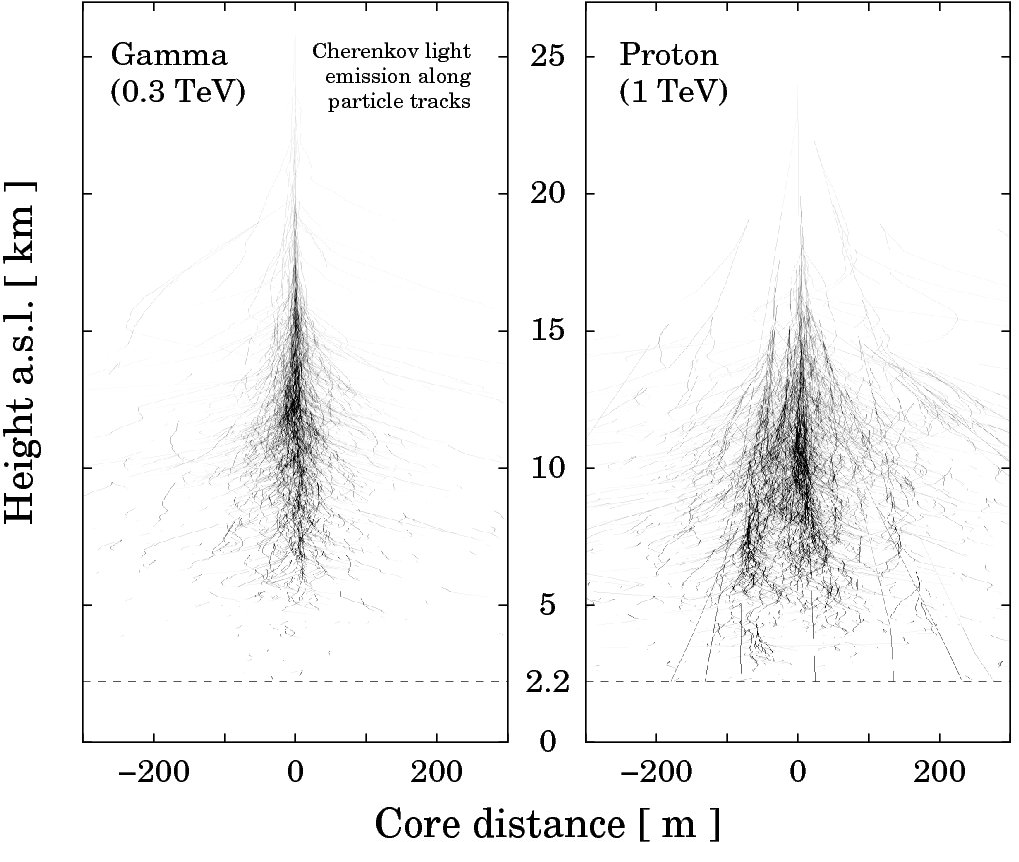
\includegraphics[width=0.95\textwidth]{images/showers_gamma_proton}
    \caption[Gamma Ray and Proton Showers]{
      A gamma ray shower alongside a proton shower~\cite{Bernlohr2008149}.
    }
    \label{fig:gamma_vs_proton_airshower}
  \end{figure}
  
  \FloatBarrier

  {\color{red}(The pp interaction doesn't always produce pions, right?? First you should talk in general about Hadronic air showers and then focus on those which look like gamma rays. Why don't you start with general lines, saying that many particles are produced at different rates and in different directions, mention how that would look like and then say that some of those particles are \pio{} which produce electromagnetic showers. -orel )}
  
